%----------------------------------------------------------------------------------------
%	Header stuff that doesn't really matter...
%----------------------------------------------------------------------------------------
\documentclass[paper=letter, fontsize=11pt]{scrartcl}
\usepackage[T1]{fontenc}
\usepackage{fourier}
\usepackage[english]{babel}
\usepackage{amsmath,amsfonts,amsthm}
\usepackage{caption}
\usepackage{sectsty}
\usepackage{graphicx}
\usepackage{float}
\allsectionsfont{\normalfont\sffamily\bfseries}
\usepackage{fancyhdr}
\fancyhead[R]{Phil Crumm 804-005-575 | Connor Proctor 703-999-284}
\fancyfoot[L]{}
\fancyfoot[C]{}
\fancyfoot[R]{\thepage}
\renewcommand{\headrulewidth}{0pt}
\renewcommand{\footrulewidth}{0pt}
\setlength{\headheight}{13.6pt}

%----------------------------------------------------------------------------------------
%	Title area
%----------------------------------------------------------------------------------------

\newcommand{\horrule}[1]{\rule{\linewidth}{#1}}

\title{	
\normalfont \normalsize 
\textsc{University of California, Los Angeles} \\ [25pt]
\horrule{0.5pt} \\[0.4cm]
\Large Computer Science M152A - Digital Design Lab \\
\horrule{2pt} \\[0.5cm]
}

\author{Connor Proctor \\* 703-999-284 \\* Phillip Crumm \\*804-005-575 \\* \\*Lab 3: Floating Point Conversion}

\date{\normalsize February 11, 2014}
\usepackage[parfill]{parskip}
\begin{document}

\clearpage\maketitle
\thispagestyle{empty}
\pagebreak

%----------------------------------------------------------------------------------------
%	The body
%----------------------------------------------------------------------------------------

\section{Objective}
This laboratory's purpose is to use the Xilinx ISE program to design and test a circuit that converts a 12-bit linear encoding to a compounded 8-bit Floating Point Representation.  

\section{Overall Design}
We are given a 12-bit two's-complement input and we need a rounded 8-bit floating point output. To do this, we first convert the two's-complement representation to 12-bit sign-magnitude to make things easier to deal with. This gives us the sign bit and a 12-bit binary value that's the absolute value of original input. We can then use a primary encoder on the absolute value to determine the expontent. We then use the expontent, and info from TABLE A in the lab specification, to extract the first five bits after the last leading zero. The first four of these bits are the significand, but because of rounding issues we use the fifth bit to determine how to round the significand and the exponent. 
\begin{figure}[H]
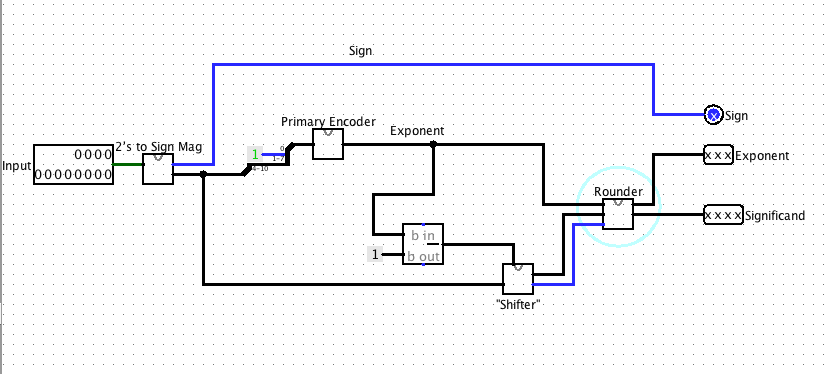
\includegraphics[height=66mm]{overall.png}
\centering
\caption{Overview}
\label{overflow}
\end{figure}

\pagebreak

\subsection{Two's complement to sign-magnitude}
Our two's complement to sign-magnitude converter sub-component takes the 12-bit input and uses inverters to invert the bits. We then use adders to add one to this to get the negation of the input. We can then use the sign bit of the input as the selector for multiplexers to decide whether to output the original input or the negation. If the sign bit is 1, we output the negation, if the sign bit is 0 we output the original input.
\begin{figure}[H]
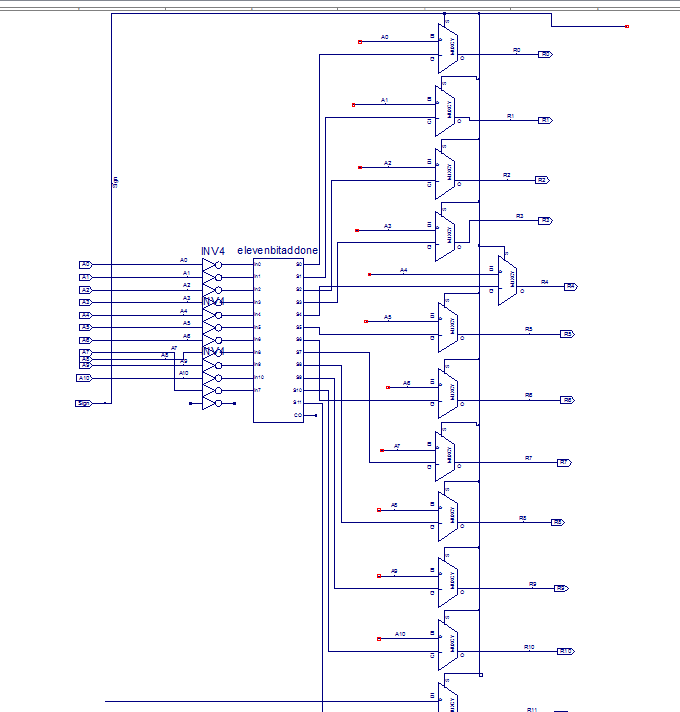
\includegraphics[height=66mm]{signmag.png}
\centering
\caption{Two's complemet to sign-magnitude}
\label{overflow}
\end{figure}

\pagebreak

\subsection{Determine Unrounded Exponent}
To determine the expontent, we designed a primary encoder. Our primary encoder first uses a system of AND gates to take the input bits and turn them all '0', except for the most significant '1'. We do this by basically ANDing every input bit with the negation of every higher bit, so that if any higher bit is 1 the AND gate outputs '0'. We then use some OR gates to convert the high bit into a binary number representation. 

In our implementatoin, the primary encoder takes 8 bits as input. The most significant seven bits are bits 4-10 from the sign-magnitude chip, and then the least significant bit is a constant '1'. This sets it up in such a way that the exponent is directly outputted. 
\begin{figure}[H]
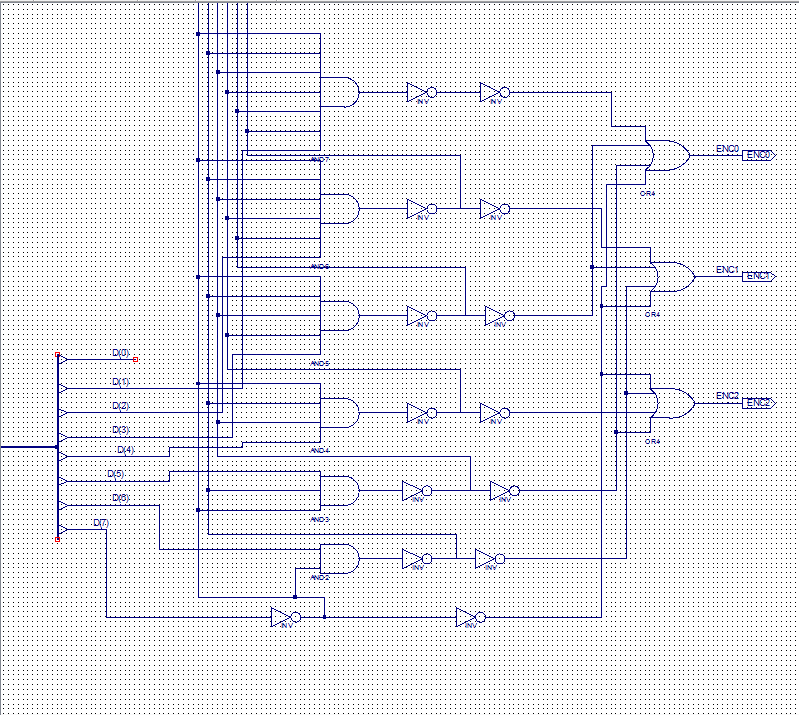
\includegraphics[height=120mm]{encoder.png}
\centering
\caption{Primary Encoder}
\label{overflow}
\end{figure}

\subsection{Extracting Significand And Rounding Bit}
To get the first five bits after the last leading zeros, we designed a component that uses multiplexers and adders to select the bits we need. In a way, it shifts the sign-magnitude output right by the exponent-1 and then selects the 5 lowest significant bits. But since we didn't need a full shifter, we just skip to those five bits. To do this, first we use the exponent-1 to select the lowest bit we want (the rounding bit), then we add 1 to the selector and input that to the next multiplexer to select the next high bit. This continues until we have the 5 bits we're looking for.
\begin{figure}[H]
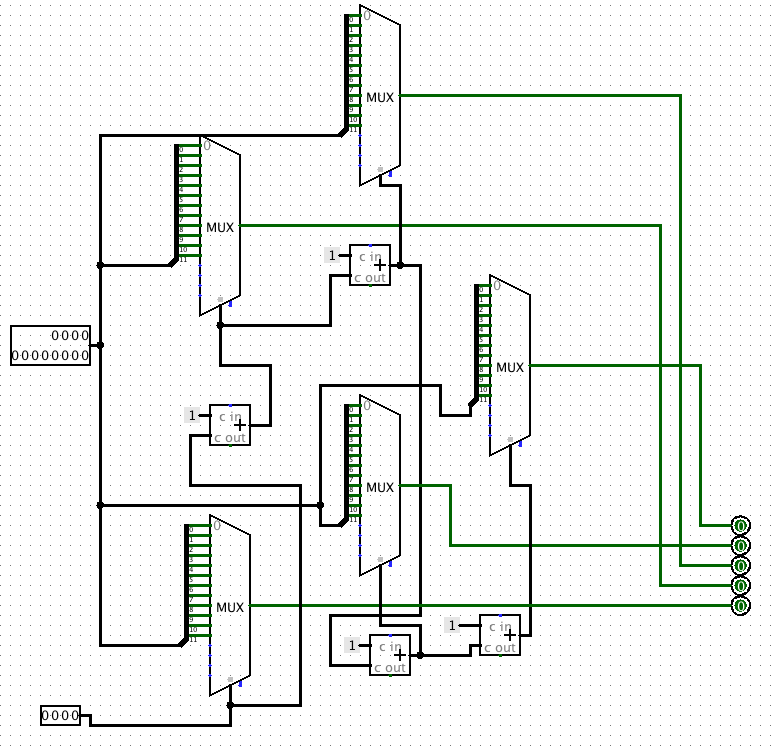
\includegraphics[height=120mm]{shifter.png}
\centering
\caption{Significand and rounding bit extractor}
\label{overflow}
\end{figure}

\pagebreak

\subsection{Rounding}
If the rounding bit (the fifth bit after the last leading zero) is 1, then we need to round up the significand. To do this, we just use a 4-bit adder to add the significand and the rounding bit. If this causes the add to overflow, producing '1' on the carryout of the adder, we must then round up the exponent. So we again use a 4 bit adder to add the carryout to the exponent. But since the significand adder overflowed, the result of the addition is '0000', but it should be '1000'. So to fix this we use a multiplexer, taking as one input the result of the addition, and as the other a constant '1000'. We use the carryout as the select bit for the multiplexer, selecting '1000' if it goes high.
\begin{figure}[H]
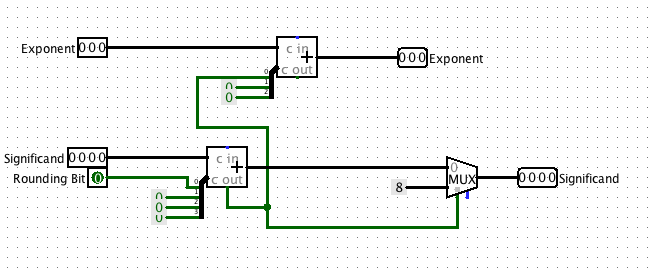
\includegraphics[height=65mm]{round.png}
\centering
\caption{Rounder}
\label{overflow}
\end{figure}

%----------------------------------------------------------------------------------------

\end{document}